\documentclass{beamer}
\usepackage{graphicx}

\title{Scaling DCEL Overlay Operations to Support Dangle and Cut Edges}
\author{Andres Oswaldo Calderon Romero}
\institute{University of California, Riverside}
\date{November 2024}

\begin{document}

\begin{frame}
    \titlepage
\end{frame}

\begin{frame}{Outline}
    \tableofcontents
\end{frame}

\section{Introduction}
\begin{frame}{Introduction}
    \begin{itemize}
        \item Extension of previous DCEL work for supporting dangle and cut edges.
        \item Introduction of a new kd-tree partitioner for overlay operations.
        \item Improvement in handling real-world datasets with scattered line segments.
        \item Overview of the partitioning strategy and overlay technique.
    \end{itemize}
\end{frame}

\begin{frame}{Motivation}
    \begin{itemize}
        \item Many applications require handling noisy or incomplete polygon data.
        \item Challenges with existing techniques in managing scattered spatial data.
        \item Need for scalability in overlay operations.
    \end{itemize}
\end{frame}

\section{Scalable Partitioning with Dangle and Cut Edges}
\begin{frame}{Kd-tree Partitioning Strategy}
    \begin{itemize}
        \item Kd-tree: Data-oriented approach using midpoint-based splits.
        \item Quadtree comparison: Space-oriented approach with uniform splits.
        \item Advantages of kd-tree in reducing empty partitions.
    \end{itemize}
\end{frame}

\begin{frame}{Overlaying Polygons with Dangle and Cut Edges}
    \begin{itemize}
        \item Extends DCEL overlay for datasets with scattered line segments.
        \item Integration of scalable polygonization for dangle and cut edges.
        \item Examples of overlay operations for applications in urban planning, advertising, and more.
    \end{itemize}
\end{frame}

\section{Experimental Evaluation}
\begin{frame}{Kd-tree vs Quadtree Performance}
    \begin{itemize}
        \item Evaluation on MainUS and GADM datasets.
        \item Comparison of tree construction, partitioning, and overlay times.
        \item Kd-tree shows improved performance with fewer empty cells.
    \end{itemize}
    \begin{figure}
        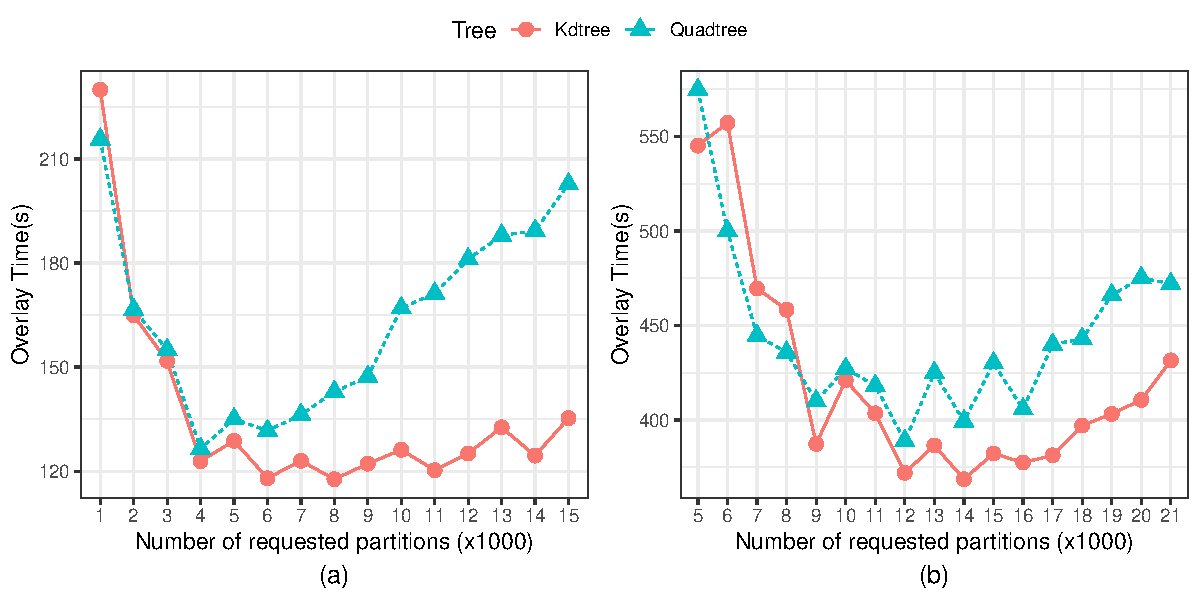
\includegraphics[width=0.8\linewidth]{chapterExtension/K/K_Overlay} % Replace with actual figure
        \caption{Kd-tree vs Quadtree performance comparison.}
    \end{figure}
\end{frame}

\begin{frame}{Overlaying Polygons with Dangle and Cut Edges}
    \begin{itemize}
        \item Comparison of overlay results across states.
        \item Performance influenced by dangle and cut edge count and intersections.
        \item Example: Texas and California with large datasets.
    \end{itemize}
    \begin{figure}
        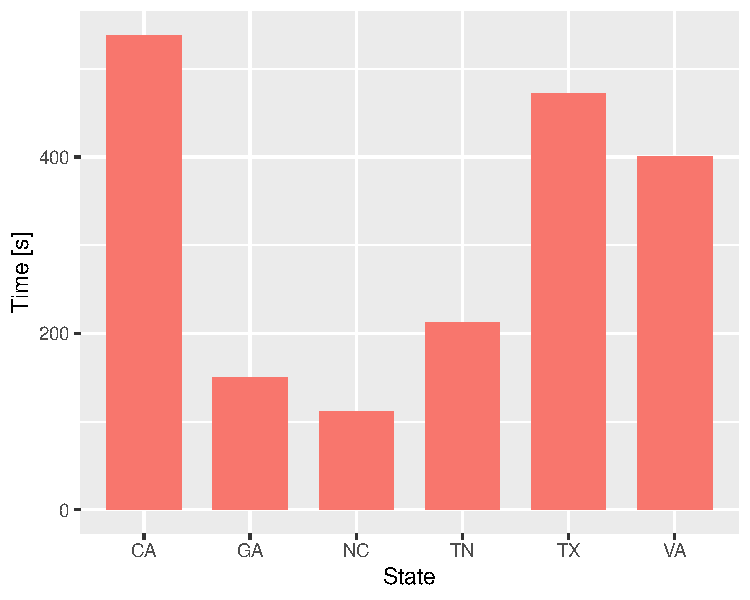
\includegraphics[width=0.5\linewidth]{chapterExtension/states} % Replace with actual figure
        \caption{Overlay performance for different states.}
    \end{figure}
\end{frame}

\section{Conclusion}
\begin{frame}{Conclusion}
    \begin{itemize}
        \item Kd-tree improves partitioning efficiency for large spatial datasets.
        \item Effective handling of scattered line segments in DCEL overlay.
        \item Scalability demonstrated in experimental evaluation.
    \end{itemize}
\end{frame}

\end{document}
